\documentclass{article}
\usepackage[utf8]{inputenc}
\usepackage{float}
\usepackage{graphicx}
\usepackage{geometry}
\usepackage{tabularx}
\usepackage{acronym}
\usepackage{listings}
\usepackage{lmodern}
\usepackage[version=4]{mhchem}
\usepackage{multicol}
\usepackage{xcolor}

\title{Systems Integration - Assignment \#1}
\date{2019/2020}

\author{João Moreira - 2015230374 \\ 
João Soares - 2009113071 }

\renewcommand{\baselinestretch}{1.3}

\begin{document}

\maketitle

\section{Introduction}

\qquad The intent of this assignment is to compare data serialization and deserialization technologies, more specifically  \ac{XML} versus \ac{gRPC}. For comparison we also implemented a \ac{JSON} serializer and deserializer and compared with the other technologies.

\section{Data Structure}

\qquad The data structure is the same in the all approaches, it consists in a car-owner many-to-one relationship, as data fields the owner has an \ac{UID}, name, telephone, address, license number, identification number and a tax number. Each vehicle has also a \ac{UID}, brand, model, body type, approval, chassis, tyre size, weight, fuel, seats, noise, co2 emissions, engine size, power, color, consumption, plate, date. In memory we stored this information as an array of owners, and each owner had its own array of vehicles. Below is a \ac{JSON} representation of the data structure used.

\section{Architecture and experiment description}

\qquad Below is a representation on how we done the development of the application and ran the experiments.

\begin{figure}[hbt!]
 \centering
 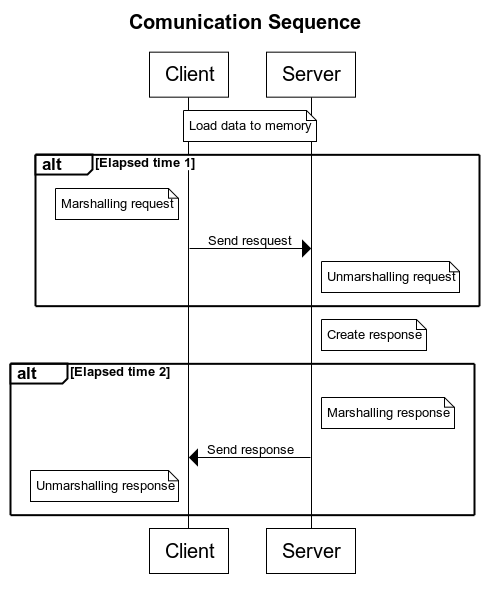
\includegraphics[scale=0.4]{Comunication_Sequence.png}
 \caption{Architecture diagram}
\end{figure}

\qquad As stated in the diagram on figure 1, at first both applications load to memory the data needed to run the experiments. To measure the performance of the different technologies we gathered the time it took to make a request/response and also the payload size after the marshalling. Since the experiments were run with both applications in the same computer, we can rule out the interference of the sending and receiving time as it is minuscule.

\qquad The elapsed time 1 is measured between the marshalling of the request to send on the client's side and the unmarshalling of the request on the server side. The elapsed time 2 is the same but with the difference that it starts measuring on the server side and finishes on the client side when the response is unmarshalled. The payload was measured after the marshalling operations.

\qquad The total time was calculated by adding the request time (elapsed time 1) with the response time (elapsed time 2).

\qquad The applications were developed and compiled with GOlang v1.13.1 and the experiments were run on a system with an Intel i5-8250U processor with 8GB Dual Channel LPDDR3 SDRAM at 1866MHz and a Samsung PM961 M.2 NVMe PCIe SSD. 

\qquad In the data used to make the experiments, we have used a sample owner with 4 vehicles and made multiple requests of the same owner, in our experiments, 100, 400, 850, 1700, 3400 and 6785 were different number of queries used per request. The 6785 number was used as an upper bound because that number of queries would account for a response with a payload of 4\ac{MB} and it is the default MAX payload size. Each of these number of queries was used to test the 3 technologies and to rule out any oscillations we ran each 100, 200, 300, 400 and 500 times and concluded the measurements stabilized at the 300 runs and above.

\qquad In terms of the actual payload per request, below is a table relating the number of queries with the final payload size when encoded in \ac{JSON}.

\begin{table}[ht]
\centering
\begin{tabular}{ c c c }
Queries & Payload Size (\ac{MB}) \\ 
100 & 0.14 \\  
400 & 0.57 \\
850 & 1.21 \\  
1700 & 2.42 \\
3400 & 4.84 \\
6785 & 9.66 \\
\end{tabular}
\caption{Payload size in \ac{JSON} per number of queries in each request}
\label{table:1}
\end{table}

\qquad All the results presented in the next section were obtained through the average of the running times of the measurements considered stable.

\section{Data Analysis}

\qquad At first lets take a look at the time it takes to marshall and unmarshall the different payload sizes.

\begin{figure}[H]
 \centering
 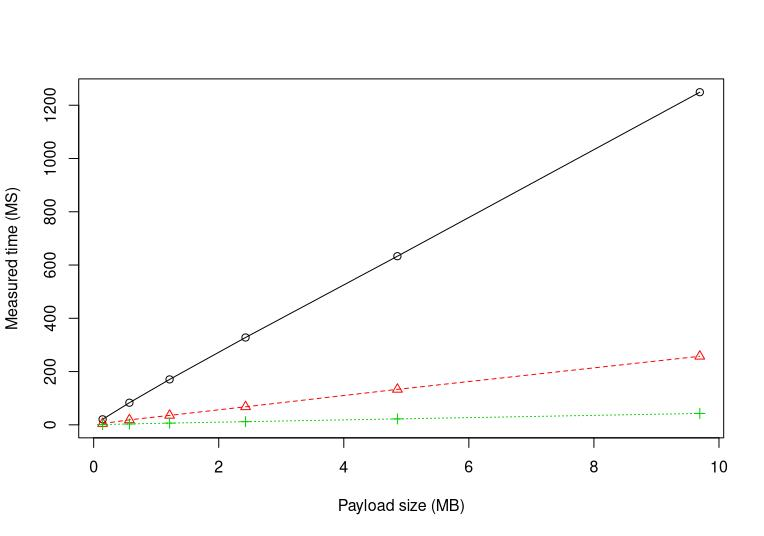
\includegraphics[scale=0.34]{totalTime.jpeg}
 \caption{Marshalling and unmarshalling time related to payload size}
\end{figure}

\qquad There is a clear difference in performance concerning the time it takes for a query to be processed, and as the payload size grows the difference between technologies also grows, being \ac{gRPC} the best of them. With this analysis we took gRPC as a reference and compared the performance improvement over the other 2 technologies, figure 3, \ac{gRPC} is 26 times faster than XML for payloads above 0.4 MB, and 5.5 times faster than JSON having the payload size no significant effect.

\begin{figure}[H]
 \centering
 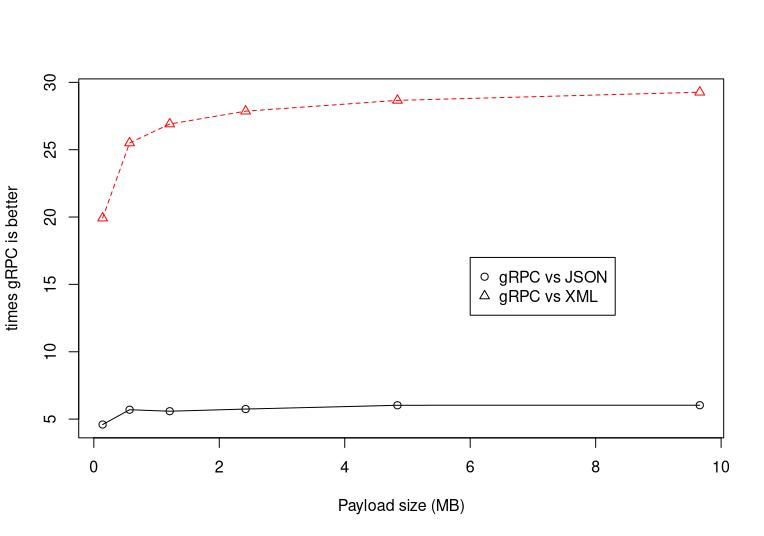
\includegraphics[scale=0.33]{gRpcVSTime.jpeg}
 \caption{Number of times gRPC is faster than JSON and XML}
\end{figure}

\qquad When looking to the final payload size, figure 4, after the marshalling \ac{gRPC} is also a more powerful technology. As stated in section 3 the reference payload size before marshalling is the \ac{JSON} objects encoded data size.

\begin{figure}[H]
 \centering
 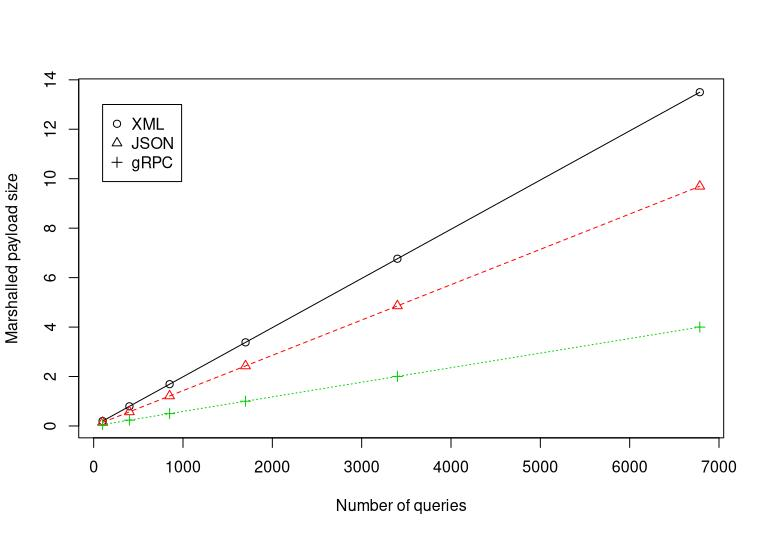
\includegraphics[scale=0.33]{payload_total_size.jpeg}
 \caption{Payload size after marshalling}
\end{figure}

\qquad When comparing gRPC with the other technologies, we can see that the average difference isn't affected at all by the payload size, as it is the same with payloads as small as 0.1MB throughout 9.7MB, as we can see in figure 5. In average the marshalled payload size in \ac{gRPC} is 2.4 times smaller than \ac{JSON} and 3.4 times smaller than \ac{XML}.

\begin{figure}[H]
 \centering
 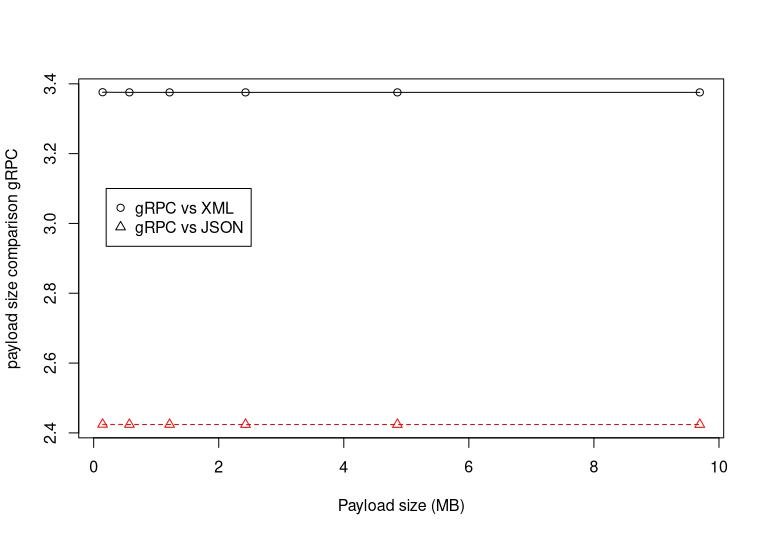
\includegraphics[scale=0.34]{payload_comp_size.jpeg}
 \caption{Difference between marshalled payload size}
\end{figure}

\qquad 

\section{Conclusion}

\qquad After this experiment we can conclude with confidence that \ac{gRPC} is a better solution in terms of processing speed on serialization operations and also in terms of the final size of resulting payload to be transmitted. This is mainly due to the fact that \ac{gRPC} uses a binary protocol format where the keys of each value are not encoded into the data as the client / server applications have the data descriptors beforehand and know the location of the values. In this case the difference we found in terms of payload size to \ac{JSON} and \ac{XML} was expected, and part of the reason for \ac{JSON} to be a bit smaller than \ac{XML} is due to the fact that it uses named closing tags for the data fields (that clearly affects the final size).

\qquad In terms of time used in the serialization operations, the same conclusion can be drawn, meaning \ac{gRPC} preforms in average 26 times faster than \ac{XML} and around 5.5 times faster than \ac{JSON}. One of main factors for such a big difference between \ac{gRPC} and \ac{XML} or even the huge gap of \ac{JSON} to \ac{XML} may be to the fact that the \ac{XML} is a less used technology in GO hence it's library is not so time optimized as the others, expetially \ac{gRPC}

\qquad On this assignment we where given a base structure to make the tests, and the time we would have needed to make more thorough testing was scarce, but it would also be interesting to make tests with different data types on the encoded data, as in this case we mainly used strings, integers and floats data types.\newline\newline

\textbf{Acronym list:}

\begin{acronym}
\acro{XML}{eXtensible Markup Language}
\acro{gRPC}{gRPC Remote Procedure Calls}
\acro{JSON}{JavaScript Object Notation}
\acro{UID}{Unique identifier}
\acro{MB}{Megabyte}
\end{acronym}


\setcounter{secnumdepth}{0}
\break
\section{Appending I - Data structure}

\qquad Example of the data structure with just one owner that owns one vehicle.

\lstset{
    string=[s]{"}{"},
    stringstyle=\color{black},
    comment=[l]{:},
    commentstyle=\color{black},
    basicstyle=\footnotesize
}
\begin{lstlisting}
{
  "Owners": [
    {
      "Uid": 1,
      "Name": "Alberto Pascoal",
      "Telephone": 321456879,
      "Address": "Coimbra, Rua Fernando Namora",
      "LicenceNumber": 5008951,
      "IdNumber": 520135478,
      "TaxNumber": 201245998,
      "Cars": [
        {
          "Uid": 1,
          "Brand": "Opel",
          "Model": "Corsa",
          "BodyType": "Van",
          "Approval": "I12309ASDSDAF51.2003",
          "Chassis": "FAIEAFSEN213ADS21",
          "TyreSize": "195/55R15",
          "Weight": 800,
          "Fuel": "Diesel",
          "Seats": 2,
          "Noise": 50,
          "Co2Emissions": 98.8,
          "EngineSize": 1700,
          "Power": 50,
          "Color": "Grey",
          "Consumption": 5.5,
          "Plate": "AA00AA",
          "Date": "01012020"
        }
      ]
    }
  ]
}
\end{lstlisting}


\end{document}
